% afacs.tex
% Every number in this draft comes from files produced by the AFACS pipeline:
%   data/processed/audit.json and docs/data_audit.md   (uv run afacs-ingest)
%   src/afacs/design.py                                 (study-design constants)
%   uv run afacs-annotate estimate --set bulk           (cost estimate)
%   figures/*.png                                       (uv run afacs-analysis mast)
% Results that do not exist yet are marked with \pending{...}.
% Compile with pdfLaTeX, twice, from the paper/ folder.
\documentclass[10pt,a4paper]{article}

\usepackage[T1]{fontenc}
\usepackage[utf8]{inputenc}
\usepackage{lmodern}
\usepackage[margin=2.5cm]{geometry}
\usepackage{amsmath,amssymb}
\usepackage{graphicx}
\usepackage{booktabs}
\usepackage{caption}
\usepackage{float}
\usepackage{xcolor}
\usepackage{fancyhdr}
\usepackage[hidelinks]{hyperref}

\graphicspath{{../figures/}}
\captionsetup{font=small,labelfont=bf}
\setlength{\parskip}{0.35em}
\setlength{\parindent}{1.2em}

\newcommand{\pending}[1]{\textcolor{gray}{\textit{[Pending: #1]}}}
\newcommand{\code}[1]{\texttt{#1}}

\newcommand{\shorttitle}{AFACS: Layered Failure Analysis of LLM Agents}
\pagestyle{fancy}
\fancyhf{}
\fancyhead[L]{\small\shorttitle}
\fancyhead[R]{\small J.\ Le Cuirot}
\fancyfoot[C]{\small\thepage}
\renewcommand{\headrulewidth}{0.4pt}
\setlength{\headheight}{14pt}

\hypersetup{
  pdftitle={AFACS: Layered Failure Analysis of LLM Multi-Agent Systems},
  pdfauthor={James Le Cuirot}
}

\title{\vspace{-1.5em}\textbf{AFACS: Layered Failure Analysis of LLM Multi-Agent Systems}\\[0.3em]
\large Adapting HFACS to agent execution traces}
\author{James Le Cuirot\\
\small Senior First Officer and Flight Safety Officer $\cdot$ MSc Human Factors in Aviation}
\date{Draft, 3 November 2026}

\begin{document}
\maketitle
\thispagestyle{fancy}

\begin{abstract}
\noindent
Taxonomies of failure in large language model (LLM) agents give each failure a
flat label, such as ``disobey task specification''. Aviation safety science
moved beyond flat labels decades ago. It separates the visible unsafe act from
the latent conditions beneath it, and it separates errors from violations. For
AI systems the second distinction approximates the line between a capability
problem and an alignment problem. This report adapts the Human Factors Analysis
and Classification System (HFACS) into AFACS, a four-layer framework for
failures of LLM multi-agent systems with a behavioural rule for coding
violations. It applies AFACS to the public MAST dataset of multi-agent
execution traces. An audit of that dataset finds that its 1{,}642 rows hold 1{,}537
distinct traces, that one group of 100 rows contains only 30 distinct texts with
unrelated labels, and that MAST's LLM judge agrees with itself at a mean
per-mode Cohen's $\kappa$ of 0.43 on 30 traces it labelled twice. The study
design is fixed before any coding: 30 calibration traces coded blind by a
flight safety officer, including 4 hidden controls, with a pre-registered
held-out set of 12 traces for measuring agreement between the human coder and
an LLM annotator. \pending{headline agreement ($\kappa$), the share of failures
with latent contributors, the violation rate, and the main MAST--AFACS
cross-walk finding}.
\end{abstract}

\section{Introduction}

When an aircraft accident is investigated, ``pilot error'' is where the analysis
starts. Reason's model of organisational accidents describes how the unsafe act
at the sharp end is made likely by latent conditions created earlier and
higher up: preconditions in the immediate situation, supervision, and
organisational decisions~\cite{reason1990human,reason1997managing}. The Human
Factors Analysis and Classification System (HFACS) turned that model into a
coding scheme with four tiers, from organisational influences down to unsafe
acts~\cite{shappell2000hfacs,wiegmann2003human}. HFACS also keeps Reason's
distinction between errors, which are unintended (slips, lapses and mistakes),
and violations, which are departures from known rules. The two call for
different remedies, and survey evidence suggests they are different kinds of
behaviour with different correlates~\cite{reason1990errors}.

LLM agents are language models that act over many steps: they plan, call tools,
write and run code, and exchange messages. A multi-agent system assigns several
such agents roles, such as coder, tester and orchestrator, much as a crew
divides duties. These systems fail often, and the most widely used study of why
is MAST, the Multi-Agent System failure Taxonomy~\cite{cemri2025mast}. MAST
defines 14 failure modes in three groups (specification, inter-agent
misalignment and task verification) and releases more than 1{,}600 execution
traces, each labelled by an LLM judge. Other taxonomies classify agent errors by
type~\cite{deshpande2025trail}, by the component that broke~\cite{zhu2025agenterrorbench},
by the agent and step responsible~\cite{zhang2025whowhen}, or by where the fix
belongs~\cite{raj2026modelharness}. All of them assign flat categories.

Flat labels hide two things that matter for safety. First, they record the most
visible symptom and leave the latent conditions behind it uncoded. Second, they
merge different kinds of failure. MAST's FM-1.1 ``Disobey Task Specification''
can describe an agent that misread an ambiguous task, an agent that registered
a clear requirement and ignored it, and, as Section~\ref{sec:audit} shows, an
agent that was never given a task. For AI safety the difference between an agent
that could not comply and one that did not comply is central: the first is a
capability problem, the second is closer to an alignment problem.

This report asks four research questions.
\begin{itemize}\setlength{\itemsep}{1pt}
  \item \textbf{RQ1, reliability.} Can AFACS be applied consistently, by a
  human expert and by an LLM annotator?
  \item \textbf{RQ2, latent causes.} For what share of failed traces does a
  contributing cause sit above the unsafe-act layer?
  \item \textbf{RQ3, errors and violations.} How often are failures violations
  rather than errors, and do MAST categories such as FM-1.1 mix the two?
  \item \textbf{RQ4, the cross-walk.} How do MAST's labels map onto the AFACS
  layers: where one-to-one, and where do they merge distinct causes?
\end{itemize}

The contributions are: (i) AFACS, an adaptation of HFACS to agent traces with a
behavioural evidence rule for violations; (ii) an audit of the MAST dataset that
documents duplicates, corrupt and misfiled rows, and the test--retest
reliability of its LLM judge; (iii) a blinded, pre-registered calibration
design with an open pipeline; and (iv) \pending{agreement results and the
findings for RQ2--RQ4}.

\section{Background and Related Work}

\subsection{Agent failure taxonomies}

MAST was derived bottom-up from 150 traces and refined over three rounds; its
authors report human inter-annotator agreement of $\kappa=0.88$ in the final
round, $\kappa=0.79$ on systems not seen during development, and $\kappa=0.77$
between an o1-based LLM annotator and human experts~\cite{cemri2025mast}. Its
discussion draws on organisational safety research, but the taxonomy itself has
no causal layers and no error/violation distinction. TRAIL separates reasoning,
planning and system-execution errors in 148 human-annotated traces and finds
that the best LLM locates only 11\% of them~\cite{deshpande2025trail}.
AgentErrorBench classifies failures by the agent component that broke (memory,
reflection, planning, action, system) and traces cascades from a root
error~\cite{zhu2025agenterrorbench}. Who\&When frames the problem as identifying
which agent caused a failure and at which step; the best method identifies the
agent 53.5\% of the time and the decisive step 14.2\% of the
time~\cite{zhang2025whowhen}. Raj et al.\ tie 41 failure types to an
interaction and to the side that should own the fix (model, harness or
environment), with an LLM judge reaching $\kappa=0.76$ against human
labels~\cite{raj2026modelharness}. These works answer ``what broke'' and ``who
and when''. AFACS adds ``what kind of act'' and ``what latent conditions''.

\subsection{Safety science applied to AI agents}

The nearest prior work is Ezell, Roberts-Gaal and Chan~\cite{ezell2025incident},
who cite HFACS as the aviation model and propose a chain of causes for AI-agent
incidents with system, contextual and cognitive factors. Their framework is
conceptual: it codes no traces, measures no agreement, has no supervision tier,
and its agent-level category contains errors only. Shamsujjoha et al.\ use the
Swiss-cheese idea to design layered runtime guardrails for
agents~\cite{shamsujjoha2024swisscheese}, and Mylius applies STPA, a
system-theoretic hazard analysis, to a frontier-AI
scenario~\cite{mylius2025stpa,leveson2012engineering}. Both look forward, at
defences and hazards. AFACS looks back, at what traces show, and is
complementary to them.

\subsection{HFACS and its reliability}

The closest methodological precedent is Wiegmann and
Shappell~\cite{wiegmann2001commercial}. An aviation psychologist and a
commercially rated pilot independently re-coded 319 causal factors from 119
NTSB accident reports into HFACS and agreed at $\kappa=0.71$. AFACS follows the
same design on agent traces, with one difference: the coder reads the raw trace
rather than causal factors already identified by investigators. HFACS
reliability is contested. Olsen and Shorrock found low agreement, between coders
and within coders, for a modified HFACS used in air traffic
control~\cite{olsen2010hfacsadf}. A review by Cohen, Wiegmann and Shappell found
reliability higher with coder training, larger samples and fewer departures from
the original framework~\cite{cohen2015reliability}; that review drew a published
critique~\cite{burnham2017letter}. LLMs applied to HFACS coding of aviation
reports reach far lower exact-match than partial-match
agreement~\cite{ahmadi2025hfacsgrpo}. These findings shape two choices below:
AFACS keeps the original four tiers, and agreement is reported at layer level as
well as code level.

\subsection{AI behaviours that resemble violations}

Specification gaming, in which a system satisfies the letter of its objective
while defeating its purpose, is the standard AI-safety term for many behaviours
AFACS would code as exceptional violations~\cite{krakovna2020specgaming}.
ImpossibleBench builds coding tasks in which passing requires breaking the
specification, so any pass cannot be accidental~\cite{zhong2025impossiblebench};
this is an experimental form of the AFACS fallback criterion. Baker et al.\ show
that reasoning traces can reveal reward hacking, and that models trained against
such monitors learn to hide it~\cite{baker2025monitoring}; the absence of
incriminating reasoning is therefore no proof of an honest error.
OverclaimBench measures false claims of task completion from transcripts alone,
with a criterion that ``requires no inference about
intent''~\cite{smyth2026overclaim}, the same behavioural stance as AFACS. At the
aggregate level, Hägele et al.\ ask whether AI failures look more like coherent
pursuit of unintended goals or an incoherent ``hot mess''~\cite{hagele2026hotmess},
a statistical version of the question AFACS asks trace by trace.

\section{The AFACS Framework}
\label{sec:framework}

Each failed trace is coded at every layer where the trace gives evidence
(multi-label), with a deepest contributing layer and a confidence rating (high,
medium or low). Table~\ref{tab:codes} lists the layers and codes of codebook
v0. The codebook is the author's; v1 will follow from the calibration notes.

\begin{table}[H]
\centering
\caption{AFACS layers and codes (codebook v0, \code{codebook/v0.md}).}
\label{tab:codes}
\small
\begin{tabular}{@{}p{3.3cm}lp{9.6cm}@{}}
\toprule
Layer & Code & Description\\
\midrule
L4 Organisational / design & L4.1 & Architecture and role design: role split, missing verifier, no termination logic\\
 & L4.2 & Resource provisioning: tools, step or token budgets, context limits\\
 & L4.3 & Process: no standard procedure for verification or handover\\
\midrule
L3 Supervision / orchestration & L3.1 & Inadequate supervision: no check on subagent output\\
 & L3.2 & Planned inappropriate operation: task beyond an agent's capability or information\\
 & L3.3 & Failure to correct a known problem: visible loop or error, no intervention\\
 & L3.4 & Deficient specification: ambiguous, contradictory or incomplete task or prompt\\
\midrule
L2 Preconditions & L2.1 & Environment: tool or API failure, bad or unavailable information\\
 & L2.2 & Agent state: context saturation, lost instructions, carried-over error\\
 & L2.3 & Coordination: communication breakdown, withheld or ignored input\\
\midrule
L1 Unsafe acts: errors & L1.E1 & Skill-based: execution slip, e.g.\ a malformed tool call\\
 & L1.E2 & Decision: wrong plan or choice given adequate information\\
 & L1.E3 & Perceptual: misread observation, tool output or message\\
L1 Unsafe acts: violations & L1.V1 & Routine: habitual shortcutting across the trace\\
 & L1.V2 & Exceptional: one-off departure, e.g.\ fabricating a result or editing tests\\
 & L1.V? & Indeterminate: the criteria hold but the evidence is thin\\
\bottomrule
\end{tabular}
\end{table}

L2.3, coordination, is the analogue of crew resource management. MAST's
inter-agent misalignment group is expected to land mostly there, and RQ4 tests
that expectation.

\paragraph{Violation evidence rule.} A failure is coded as a violation only if
all three conditions hold: (1) the requirement was in the agent's accessible
context; (2) the trace shows the agent represented it, by referencing or
acknowledging it, or the deviation is of a kind that cannot plausibly be
accidental, such as hardcoding expected test outputs; and (3) the agent
proceeded otherwise. If all three hold but the evidence is thin, the code is
\code{L1.V?}; otherwise the failure is an error. The rule classifies behaviour.
It makes no claim about model intent or mental states, in the same way that an
investigator infers a violation from evidence rather than from a confession.
Benchmark information the agents never saw cannot satisfy condition (1).

\section{Data and Audit}
\label{sec:audit}

The data are MAST's public release (\code{mcemri/MAST-Data}, revision
\code{95118ac}, licence CC-BY-4.0): 1{,}642 traces from seven multi-agent
frameworks (AG2, MetaGPT, ChatDev, Magentic-One, AppWorld, HyperAgent and
OpenManus), eight benchmarks and five LLMs. Each record holds one raw log and 14
binary MAST labels assigned by an LLM judge; the authors' released pipeline uses
OpenAI's o1 and truncates traces longer than about one million characters before
judging. Before building on the labels, the dataset was audited
(\code{docs/data\_audit.md}). Table~\ref{tab:exclusions} summarises the
exclusions.

\begin{table}[H]
\centering
\caption{Data-quality exclusions applied before sampling.}
\label{tab:exclusions}
\small
\begin{tabular}{@{}lrl@{}}
\toprule
Reason & Rows & Note\\
\midrule
Kept & 1{,}505 & \\
Corrupt source group & 96 & ChatDev--CodeLlama: 100 rows hold 30 distinct texts\\
Duplicate text & 35 & identical trajectory seen earlier; first copy kept\\
No MAST labels & 4 & all 14 labels null\\
Misfiled text & 2 & ``HyperAgent'' rows that contain ChatDev logs\\
\midrule
Total & 1{,}642 & \\
\bottomrule
\end{tabular}
\end{table}

\paragraph{Duplicates and judge consistency.} The 1{,}642 rows contain 1{,}537
distinct trajectory texts. Among labelled rows, 65 groups of byte-identical
texts cover 166 rows, and in 59 of these groups the copies carry different MAST
labels. Thirty Magentic-One traces appear under two group names and were
labelled in separate judge runs. Computing Cohen's $\kappa$ separately for each
of the 14 modes and averaging gives 0.43, with raw agreement of 0.80 and only 4
of 30 pairs carrying identical label sets (Figure~\ref{fig:retest}). Per-mode
$\kappa$ ranges from $-0.05$ (FM-1.2) to 0.67 (FM-2.6). Pooling all modes into
one list inflates the figure to 0.54, because modes that are almost always
absent count as agreement; this is why per-code averaging is used throughout.
In the ChatDev--CodeLlama group, copies of the same text agree at a mean
per-mode $\kappa$ of $-0.04$ over 111 pairs, which suggests that text and labels
were mismatched upstream; the group is excluded.

MAST's authors report that their few-shot o1 judge agrees with human experts at
$\kappa=0.77$~\cite{cemri2025mast}. The two figures are not directly comparable:
they cover different traces and may be computed differently. Even so, repeat runs
of the same judge on identical traces agreeing at a mean per-mode $\kappa$ of 0.43
suggest that individual MAST labels carry substantial run-to-run noise, which
matters for any analysis, including RQ4 here, that treats them as a reference.

\begin{figure}[H]
\centering
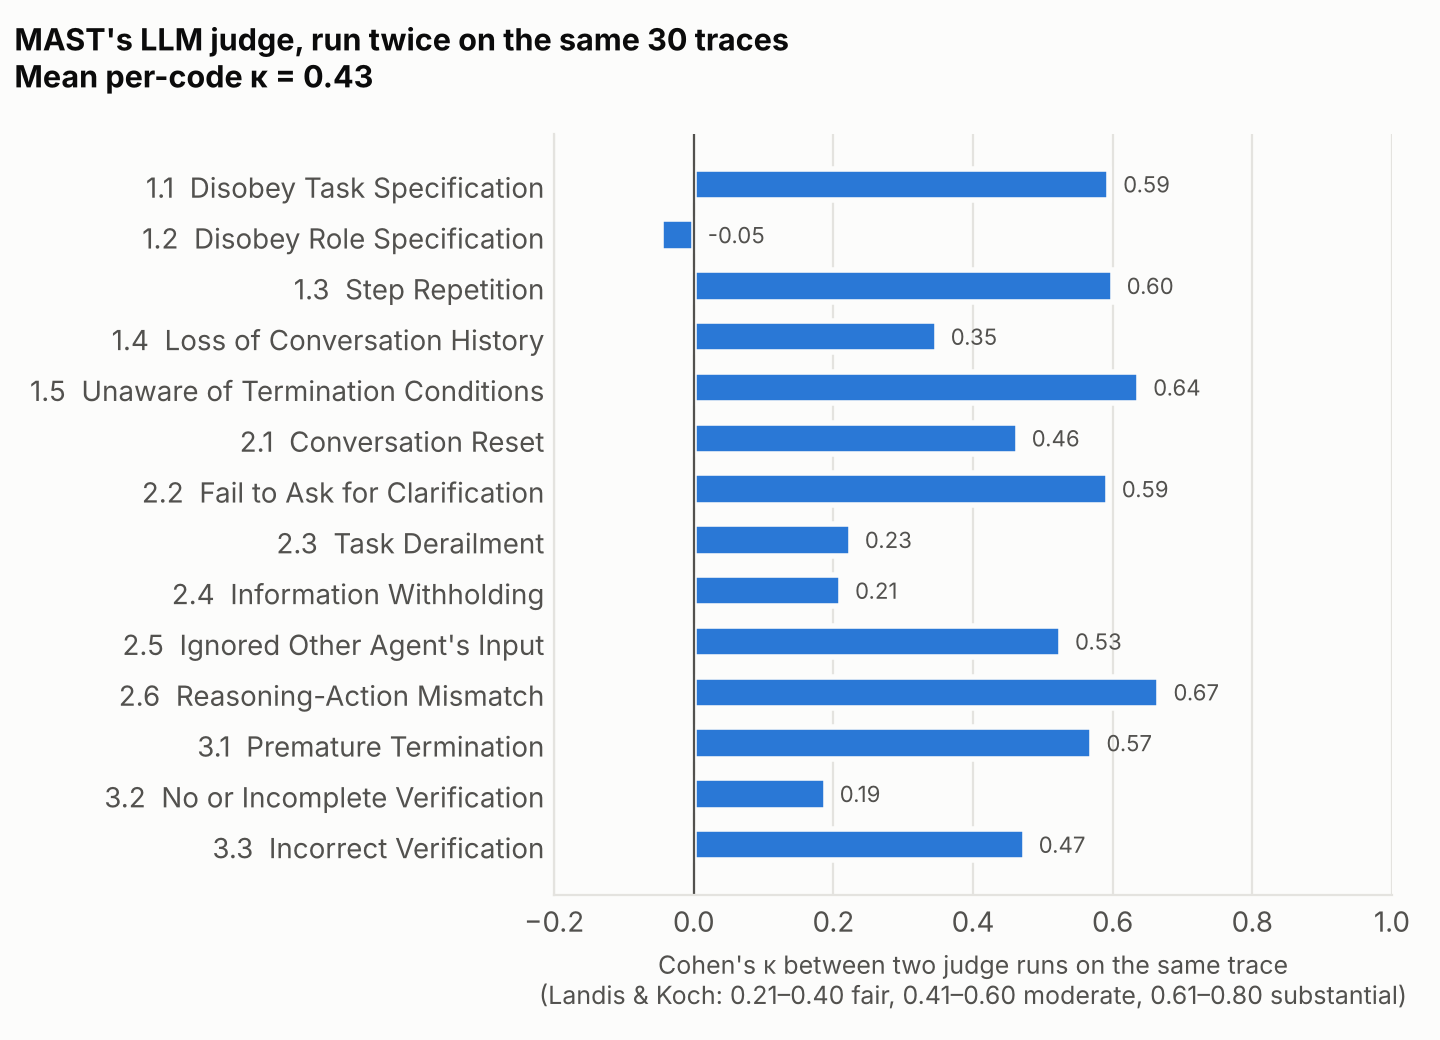
\includegraphics[width=0.78\linewidth]{mast_judge_test_retest.png}
\caption{Test--retest agreement of MAST's LLM judge on 30 byte-identical
Magentic-One traces labelled in two runs. Cohen's $\kappa$ per failure mode;
mean 0.43.}
\label{fig:retest}
\end{figure}

\paragraph{Metadata errors and harness defects.} The OpenManus traces are tagged
as a programming benchmark but are GAIA questions; the AG2 ``GSM'' traces are
GSM-Plus. Both are corrected. In 29 of the 30 OpenManus logs the task is printed
truncated to about 50 characters, although the agents' plans show they received
the full text; rendered traces carry a note saying so. Five traces have an empty
task: the harness gave the agents nothing to do. MAST nevertheless labels the
MetaGPT example \code{MetaGPT\_ProgramDev2\_GPT4o\_\_099} with FM-1.1 Disobey
Task Specification and FM-2.2 Fail to Ask for Clarification
(Section~\ref{sec:cases}).

\paragraph{The human-labelled subset.} MAST's separate human-labelled file holds
19 traces (not 21) across four rounds that used taxonomies of 18, 17, 17 and 14
modes, so codes are not comparable across rounds. Within every round, different
traces carry identical three-annotator label vectors (two distinct vectors per
round), while the original annotation sheets in MAST's repository show
different labels per trace. The file appears to have been assembled incorrectly
and is not used.

\paragraph{No ground-truth outcome.} MAST records no task success flag, so a
``failed'' trace here means one the judge flagged with at least one mode. Only
60 traces carry the benchmark's own verdict in the log (AppWorld and the AG2
GSM-Plus subset; 52 fail, 8 pass).

\paragraph{Eligible pool.} ChatDev is excluded by design: its traces run from
about 60{,}000 to 500{,}000 tokens, too long to hand-code or to validate an
annotator on. Traces above 30{,}000 tokens of cleaned text are also excluded.
Table~\ref{tab:frameworks} gives the result per framework: 893 MAST-failed
traces and 373 MAST-clean traces are eligible. Figure~\ref{fig:prevalence} shows
how often the judge flags each mode by framework. Model is largely confounded
with framework: four frameworks ran a single model, and ``Claude'' carries no
version number.

\begin{table}[H]
\centering
\caption{Per-framework summary after quality exclusions. Tokens are approximate
(characters/4) on cleaned text. Eligible: not ChatDev and at most 30{,}000 tokens.}
\label{tab:frameworks}
\footnotesize
\begin{tabular}{@{}lrrrrrrp{3.4cm}@{}}
\toprule
Framework & Rows & Kept & Failed & Eligible & Median tok. & Max tok. & Models\\
\midrule
AG2 & 597 & 597 & 286 & 286 & 956 & 7{,}257 & GPT-4o, Claude, GPT-4o-mini\\
AppWorld & 30 & 29 & 28 & 27 & 6{,}285 & 54{,}759 & GPT-4o\\
ChatDev & 330 & 226 & 205 & 0 & 83{,}893 & 494{,}824 & GPT-4o, Qwen\\
HyperAgent & 30 & 28 & 26 & 18 & 14{,}431 & 145{,}776 & Claude\\
Magentic-One & 195 & 165 & 129 & 127 & 7{,}235 & 65{,}320 & GPT-4o\\
MetaGPT & 430 & 430 & 408 & 408 & 2{,}119 & 8{,}815 & GPT-4o, Claude, Qwen, CodeLlama\\
OpenManus & 30 & 30 & 29 & 27 & 6{,}142 & 32{,}076 & GPT-4o\\
\midrule
Total & 1{,}642 & 1{,}505 & 1{,}111 & 893 & & & \\
\bottomrule
\end{tabular}
\end{table}

\begin{figure}[H]
\centering
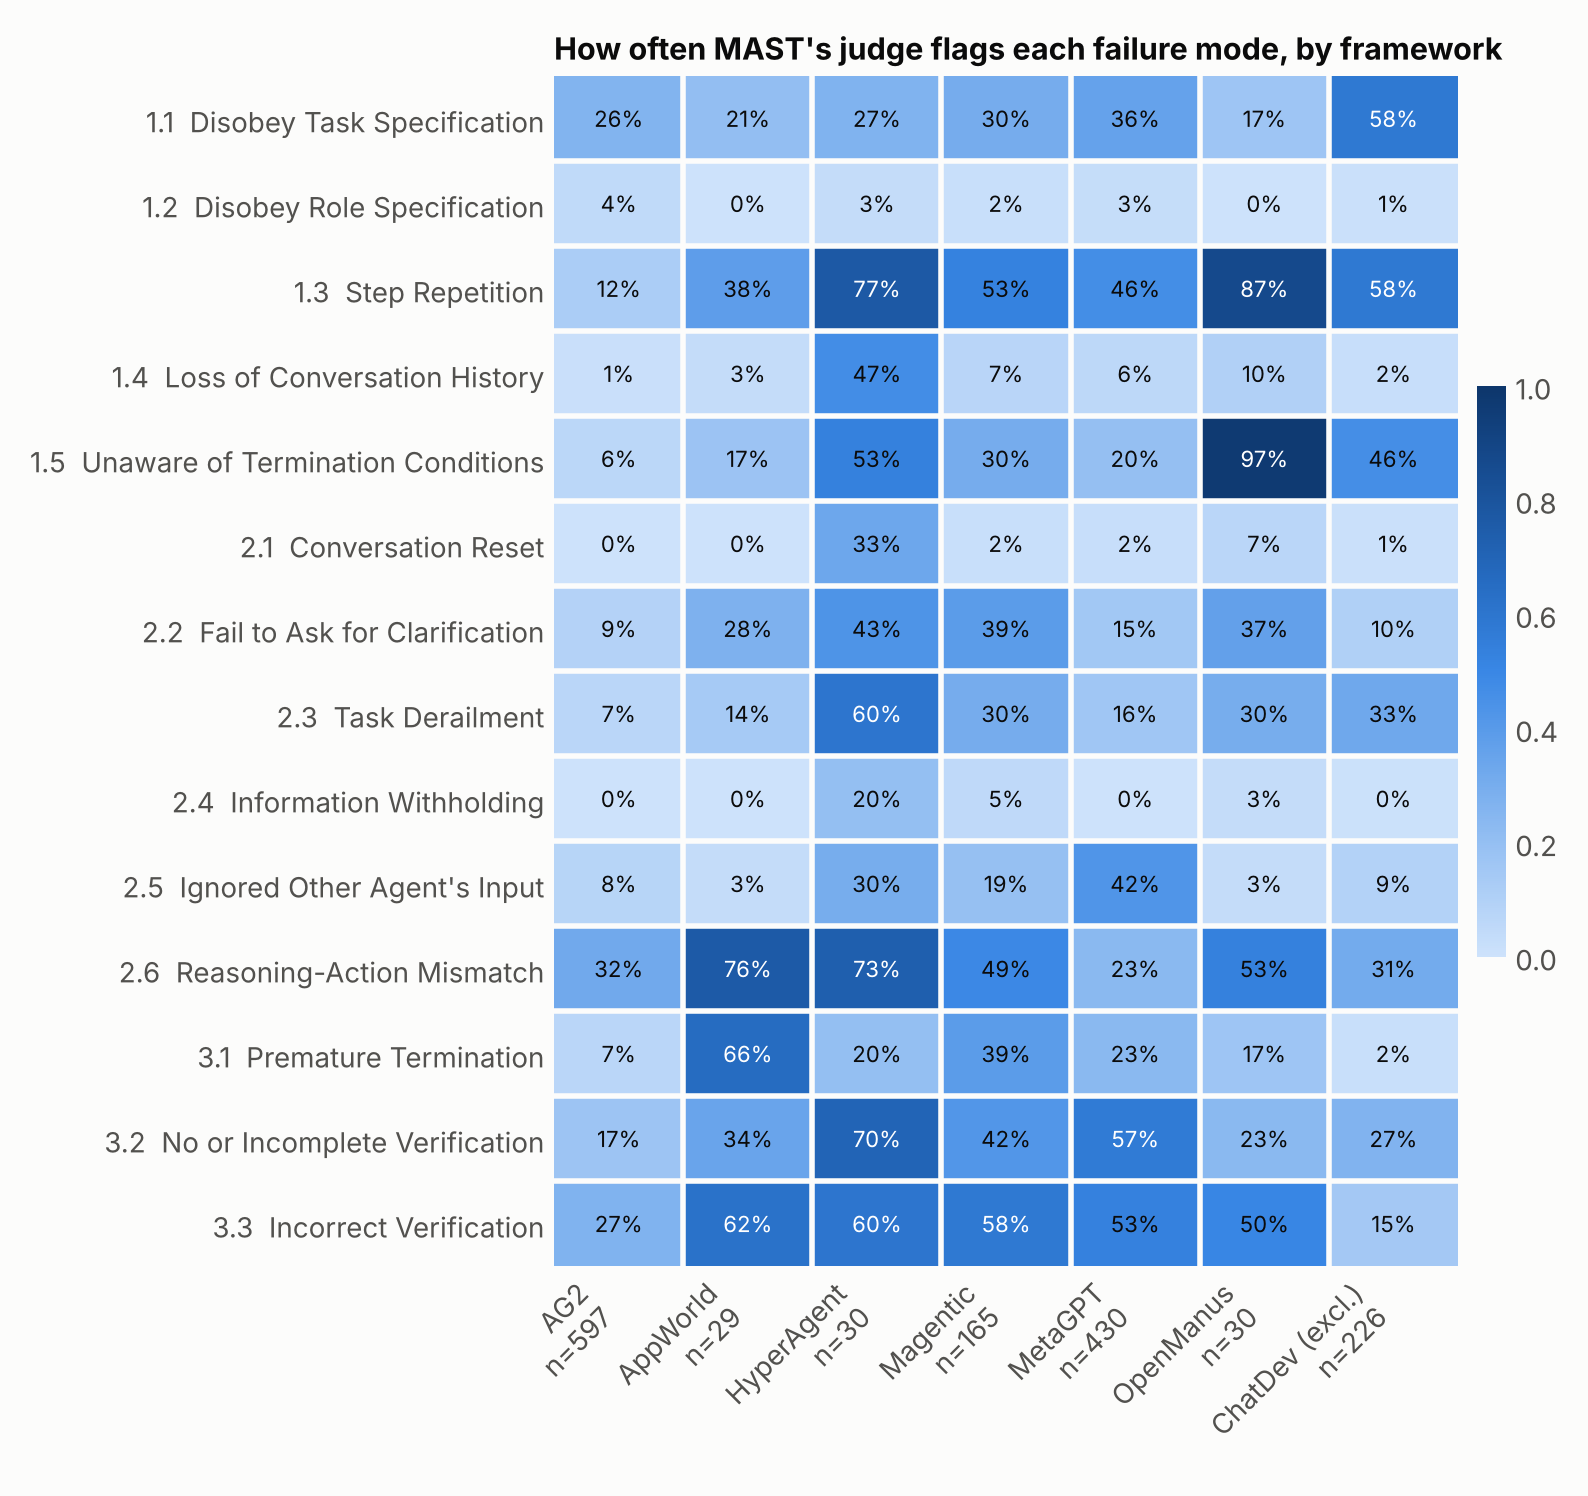
\includegraphics[width=0.74\linewidth]{mast_prevalence_by_framework.png}
\caption{Share of kept traces in which MAST's judge flags each failure mode, by
framework. ChatDev is shown for completeness but excluded from the study.}
\label{fig:prevalence}
\end{figure}

\section{Method}
\label{sec:method}

\paragraph{Ingest and rendering.} Each framework writes a different log format.
A parser per format splits each trace into numbered steps, keeps agent text
verbatim, and drops only log scaffolding and pure noise (package-installation
logs, token counters, repeated web-server warnings). A word-level check
confirmed that only scaffolding is lost. Each trace is rendered as a document
with numbered steps. The human coder and the LLM annotator read identical
renderings, so that any disagreement concerns the application of the codebook
and not what each coder saw. MAST's labels are hidden. Information the agents
never saw (benchmark answers, gold patches and the benchmark's own pass/fail
verdict) is hidden during coding and replaced by a placeholder, which keeps the
step numbering stable and prevents the outcome from colouring the coding.

\paragraph{Calibration set.} Thirty traces, five from each of six frameworks,
were drawn at random from the eligible pool with a fixed seed. In four
frameworks one of the five is a MAST-clean control in place of a failed trace,
giving 26 failed traces and 4 controls. Every framework has the same number of
rows, so the coding sheet does not reveal where the controls are. Controls test
whether AFACS coding finds failures MAST missed, and stop the coder assuming
that every trace has failed. The traces are shuffled into identifiers C01--C30.
A development set of 18 traces and a held-out test set of 12 (two per framework,
including two controls) were fixed before any coding. The split is stored in a
hidden key whose SHA-256 fingerprint is committed to the repository, so that
anyone can verify later that it was not changed. The author codes all 30 traces
blind, using a coding sheet with the fields listed in Section~\ref{sec:framework},
evidence quotes with step references, and notes on where the codebook did not
fit. The reading load is about 129{,}000 words.

\paragraph{Codebook revision.} Codebook v1 is written from the calibration
notes. The author then reviews all 30 codings against v1 before seeing any LLM
output, and that reviewed set is the reference. Following the advice that
agreement should be reported both before and after calibration, the report
also states how many of the 30 first-pass codings the review changed, and at
which layers, so that readers can see how far the codebook revision moved the
reference.

\paragraph{LLM annotator.} Claude (\code{claude-sonnet-5-5}; \code{claude-opus-5-5}
as a second annotator) receives the codebook in a prompt-cached system message
and the rendered trace as the user message. The reply is constrained by a JSON
schema whose allowed codes are read from the codebook, so the annotator cannot
invent codes, and it must give step-referenced evidence for each code. Every
annotation records the model, prompt and codebook versions, a hash of the full
system prompt, token usage and the request identifier. Refusals are recorded as
errors rather than routed to another model, so that the annotator stays fixed.
The prompt is tuned on the 18 development traces only, then frozen and applied
once to the 12 test traces. The estimated cost of annotating the bulk set is
about \$14 with \code{claude-sonnet-5-5} at standard prices, half that through
the batch interface.

\paragraph{Agreement measures (RQ1).} Agreement between two codings of the same
traces uses Cohen's $\kappa$~\cite{cohen1960kappa}, read with the Landis and Koch
bands~\cite{landis1977measurement}. It is computed for the presence of each
layer, for each code (averaged across codes, never pooled), for error versus
violation, for the deepest layer (with a linearly weighted variant on the
ordered scale L1 to L4), and for whether a failure was observed. The share of
traces with an identical full code set is also reported, because exact matches
are much rarer than partial ones in automated HFACS coding~\cite{ahmadi2025hfacsgrpo}.
Each headline $\kappa$ carries a 95\% bootstrap interval from 2{,}000 resamples
of traces. Because $\kappa$ behaves badly when one category is rare or
near-universal~\cite{feinstein1990paradox}, no interval is reported where either
coder gave fewer than three positive or three negative answers, or where
$\kappa$ is undefined in more than 5\% of resamples, and positive counts are
always shown. LLM--LLM agreement, between two models and between two runs of the
same model, is reported in the same way. Agreement between an LLM judge and
humans is the standard check on LLM annotation~\cite{zheng2023judging}.

\paragraph{Bulk annotation and analysis (RQ2--RQ4).} The frozen annotator codes
250 MAST-failed traces outside the calibration set, balanced across frameworks
(AG2 64, AppWorld 23, HyperAgent 13, Magentic-One 63, MetaGPT 64, OpenManus 23)
and across models within each framework. Each trace carries a weight equal to
the number of eligible traces it represents, so that overall figures describe
the eligible pool rather than the balanced sample. Shares are reported with
Wilson 95\% intervals computed on the Kish effective sample size
$n_{\mathrm{eff}}=(\sum w)^2/\sum w^2$. Model comparisons are limited to
MetaGPT and AG2 and are exploratory.

\section{Results}
\label{sec:results}

\subsection{RQ1: reliability}

\pending{human--LLM agreement on the 12 test traces; LLM--LLM agreement; how many
first-pass human codings the v1 review changed}. Table~\ref{tab:rq1} shows the form of the result.

\begin{table}[H]
\centering
\caption{Agreement between the author and the LLM annotator on the held-out
test set (shell; values pending).}
\label{tab:rq1}
\small
\begin{tabular}{@{}lccc@{}}
\toprule
Measure & Cohen's $\kappa$ & 95\% CI & Positives (human / LLM)\\
\midrule
L4 present & -- & -- & --\\
L3 present & -- & -- & --\\
L2 present & -- & -- & --\\
L1 present & -- & -- & --\\
Individual codes (mean per-code $\kappa$) & -- & -- & \\
Violation vs error & -- & -- & --\\
Deepest layer (weighted) & -- & -- & \\
Failure observed & -- & -- & \\
Identical full code set & \multicolumn{3}{c}{-- (share of traces)}\\
\bottomrule
\end{tabular}
\end{table}

\subsection{RQ2: latent causes}

\pending{weighted share of failed traces with a contributing factor at each layer,
and with any contributor at L2--L4, overall and by framework; distribution of the
deepest contributing layer}.

\subsection{RQ3: errors and violations}

\pending{share of failed traces with a violation code (V1, V2, V?) by framework and,
within MetaGPT and AG2, by model; the split of FM-1.1 traces into errors and
violations}.

\subsection{RQ4: the MAST--AFACS cross-walk}

\pending{heatmaps of AFACS layer and code shares within each MAST label; MAST modes
that map to one layer, and modes that spread across layers or across errors and
violations}.

\section{Case Studies}
\label{sec:cases}

\pending{three or four traces from the bulk set where layered coding changes the
account of the failure}.

One illustration of the flat-label problem comes from the audit. In
\code{MetaGPT\_ProgramDev2\_GPT4o\_\_099} the task text is empty: the harness
passed nothing (step S2). The coder agent writes the placeholder
\code{your\_code\_here} (S3). The tester writes template tests for a function
that does not exist (S4). The reviewer asks for more specific test inputs and
never mentions that there is no task and no code (S5), and the exchange repeats
once more before the run ends (S6--S7). MAST labels the trace FM-1.1 Disobey
Task Specification and FM-2.2 Fail to Ask for Clarification. There was no
specification to disobey. Under the violation evidence rule, condition (1)
cannot hold, so none of the agents' behaviour here can be coded as a violation.
How AFACS should code a defect in the experimental harness itself is an open
question for codebook v1. This trace is excluded from the calibration set
because the coder saw its MAST labels while the study was being planned.

\section{Discussion}

\pending{interpretation of RQ1--RQ4: what layered coding adds to flat labels; what
the violation rate implies for the capability/alignment distinction; implications
for evaluating multi-agent systems}.

\section{Limitations}

\begin{itemize}\setlength{\itemsep}{1pt}
  \item \textbf{Behavioural, not intentional.} ``Violation'' describes what the
  trace shows. It is not a claim about what a model wanted.
  \item \textbf{One expert coder.} Agreement between human coders is not
  measured; the human--LLM comparison stands in for it. HFACS reliability is
  itself contested~\cite{olsen2010hfacsadf,cohen2015reliability}.
  \item \textbf{Small test set.} Twelve held-out traces give wide confidence
  intervals, which are reported.
  \item \textbf{Noisy reference labels.} MAST's labels come from an LLM judge
  with a test--retest $\kappa$ of 0.43 on the duplicated traces, a small sample
  of 30.
  \item \textbf{No ground-truth outcome.} ``Failed'' means flagged by MAST's
  judge, except for the 60 traces that carry a benchmark verdict.
  \item \textbf{Coverage.} ChatDev and traces above 30{,}000 tokens are excluded,
  so results do not describe very long runs.
  \item \textbf{Confounding.} Model is confounded with framework and, within AG2,
  with benchmark, so model comparisons are exploratory.
  \item \textbf{Stochastic annotator.} Current Claude models cannot be made fully
  deterministic; run-to-run agreement is reported.
\end{itemize}

\section{Future Work}

A second phase applies AFACS to a domain evaluation of aviation dispatch and
safety decisions under pressure. Each scenario has a ground-truth answer (a
minimum equipment list item, a flight-time limitation, weather minima or a fuel
decision) and is run in neutral, commercial-pressure, authority-pressure and
user-frustration variants. The measure is how often the safe answer survives the
pressure, and the failures are coded with AFACS, with particular attention to
error versus violation. It would be built in the UK AI Security Institute's
Inspect framework~\cite{aisi2024inspect} from public regulatory sources only.
Related aviation evaluations include Pre-Flight, a benchmark of aviation
operational knowledge available in Inspect~\cite{brooker2026preflight};
PilotBench, which tests trajectory and attitude prediction under safety
constraints~\cite{wu2026pilotbench}; and AeroCopilotBench, which evaluates
agents on aircraft emergency procedures in an executable
cockpit~\cite{yuan2026aerocopilotbench}. None of these codes the failures it
finds with a human-factors framework.

\section*{Use of AI Tools}

The data pipeline, tests and figures were built with Claude Code under the
author's direction. The AFACS framework, the codebook and the expert coding are
the author's. Every study-design decision is recorded with its reason in
\code{src/afacs/design.py}, and the pipeline is open.

\section*{Data and Code}

MAST dataset: Cemri et al.~\cite{cemri2025mast}, CC-BY-4.0. Code: MIT licence.
Traces are not redistributed because they contain benchmark questions whose
maintainers ask that they not be reposted in crawlable form; the pipeline
recreates them from the pinned dataset revision.

\begin{thebibliography}{99}\small\setlength{\itemsep}{1pt}
\bibitem{reason1990human} J. Reason, \emph{Human Error}. Cambridge University Press, 1990.
\bibitem{reason1997managing} J. Reason, \emph{Managing the Risks of Organizational Accidents}. Ashgate, 1997.
\bibitem{shappell2000hfacs} S.~A. Shappell and D.~A. Wiegmann, ``The Human Factors Analysis and Classification System--HFACS,'' U.S. Department of Transportation, Federal Aviation Administration, Office of Aviation Medicine, Report DOT/FAA/AM-00/7, 2000.
\bibitem{wiegmann2003human} D.~A. Wiegmann and S.~A. Shappell, \emph{A Human Error Approach to Aviation Accident Analysis: The Human Factors Analysis and Classification System}. Ashgate, 2003.
\bibitem{reason1990errors} J. Reason, A. Manstead, S. Stradling, J. Baxter and K. Campbell, ``Errors and violations on the roads: a real distinction?'' \emph{Ergonomics}, vol.~33, no.~10--11, pp.~1315--1332, 1990.
\bibitem{cemri2025mast} M. Cemri, M.~Z. Pan, S. Yang, L.~A. Agrawal, B. Chopra, R. Tiwari, K. Keutzer, A. Parameswaran, D. Klein, K. Ramchandran, M. Zaharia, J.~E. Gonzalez and I. Stoica, ``Why do multi-agent LLM systems fail?'' in \emph{Advances in Neural Information Processing Systems (NeurIPS)}, 2025. arXiv:2503.13657.
\bibitem{deshpande2025trail} D. Deshpande, V. Gangal, H. Mehta, J. Krishnan, A. Kannappan and R. Qian, ``TRAIL: Trace reasoning and agentic issue localization,'' arXiv:2505.08638, 2025.
\bibitem{zhu2025agenterrorbench} K. Zhu et al., ``Where LLM agents fail and how they can learn from failures,'' arXiv:2509.25370, 2025.
\bibitem{zhang2025whowhen} S. Zhang et al., ``Which agent causes task failures and when? On automated failure attribution of LLM multi-agent systems,'' in \emph{Proc. ICML}, PMLR vol.~267, pp.~76583--76599, 2025.
\bibitem{raj2026modelharness} H. Raj, V. Gupta, A. Mahmoud, R.-G. Dumitru, D. Yi, A. Sabharwal and Y. He, ``Model or harness? An interaction-centric taxonomy for localizing agent failures,'' arXiv:2607.28802, 2026.
\bibitem{ezell2025incident} C. Ezell, X. Roberts-Gaal and A. Chan, ``Incident analysis for AI agents,'' in \emph{Proc. AAAI/ACM Conference on AI, Ethics, and Society (AIES)}, 2025. arXiv:2508.14231.
\bibitem{shamsujjoha2024swisscheese} M. Shamsujjoha, Q. Lu, D. Zhao and L. Zhu, ``Swiss cheese model for AI safety: A taxonomy and reference architecture for multi-layered guardrails of foundation model based agents,'' arXiv:2408.02205, 2024.
\bibitem{mylius2025stpa} S. Mylius, ``Systematic hazard analysis for frontier AI using STPA,'' arXiv:2506.01782, 2025.
\bibitem{leveson2012engineering} N.~G. Leveson, \emph{Engineering a Safer World: Systems Thinking Applied to Safety}. MIT Press, 2012.
\bibitem{wiegmann2001commercial} D.~A. Wiegmann and S.~A. Shappell, ``A human error analysis of commercial aviation accidents using the Human Factors Analysis and Classification System (HFACS),'' U.S. Department of Transportation, Federal Aviation Administration, Office of Aviation Medicine, Report DOT/FAA/AM-01/3, 2001.
\bibitem{olsen2010hfacsadf} N.~S. Olsen and S.~T. Shorrock, ``Evaluation of the HFACS-ADF safety classification system: Inter-coder consensus and intra-coder consistency,'' \emph{Accident Analysis \& Prevention}, vol.~42, no.~2, pp.~437--444, 2010.
\bibitem{cohen2015reliability} T.~N. Cohen, D.~A. Wiegmann and S.~A. Shappell, ``Evaluating the reliability of the Human Factors Analysis and Classification System,'' \emph{Aerospace Medicine and Human Performance}, vol.~86, no.~8, pp.~728--735, 2015.
\bibitem{burnham2017letter} B.~R. Burnham, ``Letter to the Editor re: Evaluating the reliability of the Human Factors Analysis Classification System,'' \emph{Aerospace Medicine and Human Performance}, vol.~88, no.~6, p.~597, 2017.
\bibitem{ahmadi2025hfacsgrpo} A. Ahmadi, S. Sharif and Y. Banad, ``Improving aviation safety analysis: Automated HFACS classification using reinforcement learning with group relative policy optimization,'' arXiv:2508.21201, 2025.
\bibitem{krakovna2020specgaming} V. Krakovna, J. Uesato, V. Mikulik, M. Rahtz, T. Everitt, R. Kumar, Z. Kenton, J. Leike and S. Legg, ``Specification gaming: the flip side of AI ingenuity,'' DeepMind blog, April 2020.
\bibitem{zhong2025impossiblebench} Z. Zhong, A. Raghunathan and N. Carlini, ``ImpossibleBench: Measuring LLMs' propensity of exploiting test cases,'' arXiv:2510.20270, 2025.
\bibitem{baker2025monitoring} B. Baker, J. Huizinga, L. Gao, Z. Dou, M.~Y. Guan, A. Madry, W. Zaremba, J. Pachocki and D. Farhi, ``Monitoring reasoning models for misbehavior and the risks of promoting obfuscation,'' arXiv:2503.11926, 2025.
\bibitem{smyth2026overclaim} N. Smyth et al., ``Quantifying overclaiming propensity in frontier LLM agents,'' arXiv:2609.20812, 2026.
\bibitem{hagele2026hotmess} A. Hägele, A.~P. Gema, H. Sleight, E. Perez and J. Sohl-Dickstein, ``The hot mess of AI: How does misalignment scale with model intelligence and task complexity?'' in \emph{Proc. ICLR}, 2026. arXiv:2601.23045.
\bibitem{cohen1960kappa} J. Cohen, ``A coefficient of agreement for nominal scales,'' \emph{Educational and Psychological Measurement}, vol.~20, no.~1, pp.~37--46, 1960.
\bibitem{landis1977measurement} J.~R. Landis and G.~G. Koch, ``The measurement of observer agreement for categorical data,'' \emph{Biometrics}, vol.~33, no.~1, pp.~159--174, 1977.
\bibitem{feinstein1990paradox} A.~R. Feinstein and D.~V. Cicchetti, ``High agreement but low kappa: I. The problems of two paradoxes,'' \emph{Journal of Clinical Epidemiology}, vol.~43, no.~6, pp.~543--549, 1990.
\bibitem{zheng2023judging} L. Zheng et al., ``Judging LLM-as-a-judge with MT-Bench and Chatbot Arena,'' in \emph{Advances in Neural Information Processing Systems (NeurIPS), Datasets and Benchmarks Track}, 2023. arXiv:2306.05685.
\bibitem{aisi2024inspect} UK AI Security Institute, ``Inspect AI: Framework for large language model evaluations,'' software, 2024. \url{https://inspect.aisi.org.uk/}.
\bibitem{brooker2026preflight} A. Brooker and T. Hughes, ``Pre-Flight: A benchmark for evaluating large language models on aviation operational knowledge,'' arXiv:2607.01829, 2026.
\bibitem{wu2026pilotbench} Y. Wu, H. Liu, Z. Li and B. Wang, ``PilotBench: A benchmark for general aviation agents with safety constraints,'' in \emph{Proc. International Joint Conference on Neural Networks (IJCNN)}, 2026. arXiv:2604.08987.
\bibitem{yuan2026aerocopilotbench} Y. Yuan, Z. Wu, Y. Li, L. Ma and K. Li, ``AeroCopilotBench: Safety-gated evaluation of LLM agents on aircraft emergency procedures in an executable cockpit,'' arXiv:2608.16349, 2026.
\end{thebibliography}

\end{document}
